 % =============================================================================
% Low Power Edge Inference for Green Computing:
% An Evaluation of Post-Training Quantization Techniques
% =============================================================================
% IJACSA Submission — IEEEtran two-column journal format
% Authors: Harshpreet Singh, Sameer Kumar
% Affiliation: Chitkara University, India
% =============================================================================

\documentclass[journal]{IEEEtran}

% -----------------------------------------------------------------------------
% MATH PACKAGES
% -----------------------------------------------------------------------------
\usepackage{amsmath}
\usepackage{amssymb}

% -----------------------------------------------------------------------------
% GRAPHICS AND TABLES
% -----------------------------------------------------------------------------
\usepackage{graphicx}
\usepackage{booktabs}
\usepackage{multirow}
\usepackage{array}
\usepackage{xcolor}
\usepackage{adjustbox}

% -----------------------------------------------------------------------------
% ALGORITHMS
% -----------------------------------------------------------------------------
\usepackage{algorithm}
\usepackage{algorithmic}

% -----------------------------------------------------------------------------
% HYPERLINKS AND REFERENCES
% -----------------------------------------------------------------------------
\usepackage{url}
\usepackage{cite}
\usepackage[colorlinks=true,linkcolor=blue,citecolor=blue,urlcolor=blue]{hyperref}

% -----------------------------------------------------------------------------
% LISTS AND ENUMERATIONS
% -----------------------------------------------------------------------------
\usepackage{enumitem}

% -----------------------------------------------------------------------------
% SYMBOLS AND SPECIAL CHARACTERS
% -----------------------------------------------------------------------------
\usepackage{pifont}
\usepackage{textcomp}

% -----------------------------------------------------------------------------
% PLOTS
% -----------------------------------------------------------------------------
\usepackage{pgfplots}
\pgfplotsset{compat=1.17}

% -----------------------------------------------------------------------------
% TIKZ DIAGRAMS
% -----------------------------------------------------------------------------
\usepackage{tikz}
\usetikzlibrary{arrows.meta, positioning, shapes.geometric, fit, backgrounds, calc}

% -----------------------------------------------------------------------------
% CUSTOM COMMANDS
% -----------------------------------------------------------------------------
\newcommand{\cmark}{\ding{51}}
\newcommand{\xmark}{\ding{55}}
\newcommand{\methodname}{PTQ-Edge}

% Math operators
\DeclareMathOperator*{\argmin}{arg\,min}
\DeclareMathOperator*{\argmax}{arg\,max}

% -----------------------------------------------------------------------------
% BIBLIOGRAPHY STYLE
% -----------------------------------------------------------------------------
\bibliographystyle{IEEEtran}

% =============================================================================
% DOCUMENT METADATA
% =============================================================================
\title{Low Power Edge Inference for Green Computing: An Evaluation of Post-Training Quantization on Apple Silicon}

\author{%
\begin{minipage}[t]{0.47\linewidth}
  \centering
  {\normalsize\bfseries Harshpreet Singh}\\[3pt]
  \small Chitkara University Institute of Engineering and Technology\\
  \small Chitkara University, Punjab, India\\
  \small\texttt{harshpreet393.be22@chitkara.edu.in}
\end{minipage}%
\hfill%
\begin{minipage}[t]{0.47\linewidth}
  \centering
  {\normalsize\bfseries Sameer Kumar}\\[3pt]
  \small Chitkara University Institute of Engineering and Technology\\
  \small Chitkara University, Punjab, India\\
  \small\texttt{sameer776.be22@chitkara.edu.in}
\end{minipage}%
}

\begin{document}

\maketitle

% =============================================================================
% ABSTRACT
% =============================================================================
\begin{abstract}
Running large language models on edge devices means squeezing them into tight memory budgets, without losing too much accuracy in the process. In this paper, we evaluate post-training quantization (PTQ) for small language models on Apple Silicon using Apple's MLX framework at three precision levels (FP16, INT8, INT4). We benchmark the Qwen3.5 series (0.8B, 2B, 4B parameters) and Phi-3 Mini (3.82B) on an M4 Pro with 24\,GB unified memory. INT4 gives us $2.0\times$--$3.8\times$ better throughput over FP16 and cuts memory by $3.5\times$--$3.6\times$. On the accuracy side, our logit-based full MMLU evaluation (all 57 subjects, 14,042 questions) shows that INT8 is effectively lossless for the 2B and larger models, while INT4 introduces model-dependent drops of 2.39--7.90 percentage points. Even so, the 4B-class models retain strong INT4 accuracy (69.82\% for Qwen3.5-4B and 66.97\% for Phi-3 Mini). Every model we tested fits within 2.5\,GB after INT4 quantization, which opens the door to edge deployment even on devices with only 8\,GB of RAM.
\end{abstract}

\begin{IEEEkeywords}
post-training quantization, edge inference, Apple Silicon, MLX framework, small language models, energy efficiency, MMLU, INT4, green computing
\end{IEEEkeywords}

% =============================================================================
% 1. INTRODUCTION
% =============================================================================
\section{Introduction}

Large language models (LLMs) have reshaped the way we think about natural language processing. Text generation, reasoning, and knowledge retrieval have all taken massive leaps forward \cite{brown2020language, openai2023gpt4}. But this progress comes at a cost. The International Energy Agency projects that data centers will eat up 945\,TWh of electricity per year by 2030, roughly 3\% of the world's total, with AI workloads being a major driver of that growth \cite{iea2025energyai}.

\subsection{Sustainability Challenge}

The environmental footprint of LLMs extends across their entire lifecycle. Training gets most of the attention, but inference is actually the bigger energy consumer in practice, accounting for about 60\% of total ML compute in production systems \cite{patterson2021carbon}. And as models keep getting bigger to push performance forward, energy consumption scales right along with them.

One promising direction is edge computing, which brings inference closer to the user: lower latency, better privacy, and less dependence on data center infrastructure \cite{shi2016edge}. The problem is that edge devices are resource-constrained. Most have 8--16\,GB of memory, limited compute, and tight power budgets. Just loading a 4-billion-parameter model in FP16 takes around 8\,GB of memory for weights alone, which is more than a lot of edge devices can spare.

\subsection{Quantization as a Solution}

This is where post-training quantization (PTQ) comes in. PTQ reduces weight precision from 16-bit or 32-bit floating-point down to 8-bit or even 4-bit integers \cite{han2015deep}. The key advantage over quantization-aware training (QAT) is that PTQ works directly on pre-trained weights, with no retraining needed. That makes it a natural fit for getting existing models onto edge devices.

That said, several practical questions remain unanswered:

\begin{itemize}[leftmargin=*,nosep]
    \item How do different quantization bit-widths affect throughput, memory, and accuracy on Apple Silicon?
    \item How does model size influence quantization sensitivity?
\end{itemize}

\subsection{Contributions}

We set out to answer these questions through hands-on experiments on an Apple M4 Pro. Here is what we contribute:

\begin{enumerate}[leftmargin=*,nosep]
    \item \textbf{Quantization analysis}: We benchmark MLX at three precision levels (FP16, INT8, INT4) across the Qwen3.5 series and Phi-3 Mini, measuring how each level affects throughput, memory usage, and accuracy.

    \item \textbf{Accuracy evaluation}: We use logit-based full-MMLU scoring on all 57 subjects (14,042 questions), which reduces the 95\% confidence interval around overall accuracy to about $\pm 0.8$\,pp and lets us measure quantization effects with much higher confidence.

    \item \textbf{Energy estimation}: We report CodeCarbon-based energy estimates for every configuration, while being upfront about the limitations of software-based power estimation on Apple Silicon.
\end{enumerate}

\begin{figure*}[htbp]
\centering
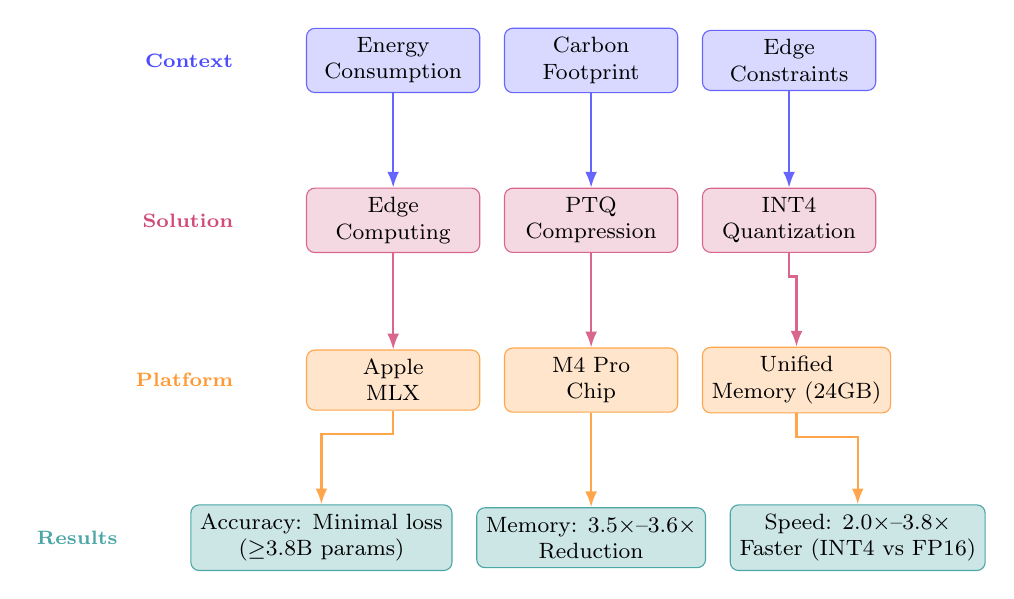
\begin{tikzpicture}[
    node distance=0.6cm and 0.3cm,
    box/.style={
        rectangle,
        rounded corners=3pt,
        draw,
        minimum width=2.2cm,
        minimum height=0.7cm,
        align=center,
        font=\footnotesize
    },
    layerbox/.style={
        rectangle,
        rounded corners=5pt,
        draw,
        thick
    },
    arrow/.style={
        -{Latex[length=2mm, width=1.5mm]},
        thick
    }
]

% === Layer 1: Context (Blue) ===
\node[box, fill=blue!15, draw=blue!60] (energy) {Energy\\Consumption};
\node[box, fill=blue!15, draw=blue!60, right=of energy] (carbon) {Carbon\\Footprint};
\node[box, fill=blue!15, draw=blue!60, right=of carbon] (edge) {Edge\\Constraints};

% === Layer 2: Solution (Purple) ===
\node[box, fill=purple!15, draw=purple!60, below=1.2cm of carbon] (ptq) {PTQ\\Compression};
\node[box, fill=purple!15, draw=purple!60, right=of ptq] (int4) {INT4\\Quantization};
\node[box, fill=purple!15, draw=purple!60, left=of ptq] (edge2) {Edge\\Computing};

% === Layer 3: Platform (Orange) ===
\node[box, fill=orange!20, draw=orange!70, below=1.2cm of ptq] (m4) {M4 Pro\\Chip};
\node[box, fill=orange!20, draw=orange!70, right=of m4] (mem) {Unified\\Memory (24GB)};
\node[box, fill=orange!20, draw=orange!70, left=of m4] (mlx) {Apple\\MLX};

% === Layer 4: Evaluation (Teal/Green) ===
\node[box, fill=teal!20, draw=teal!70, below=1.2cm of m4, minimum width=2.8cm] (memory) {Memory: 3.5$\times$--3.6$\times$\\Reduction};
\node[box, fill=teal!20, draw=teal!70, right=of memory, minimum width=2.8cm] (speed) {Speed: 2.0$\times$--3.8$\times$\\Faster (INT4 vs FP16)};
\node[box, fill=teal!20, draw=teal!70, left=of memory, minimum width=2.8cm] (energy2) {Accuracy: Minimal loss\\($\geq$3.8B params)};

% === Arrows: Context → Solution ===
\draw[arrow, blue!60] (energy.south) -- ++(0,-0.3) -| (edge2.north);
\draw[arrow, blue!60] (carbon.south) -- (ptq.north);
\draw[arrow, blue!60] (edge.south) -- ++(0,-0.3) -| (int4.north);

% === Arrows: Solution → Platform ===
\draw[arrow, purple!60] (edge2.south) -- ++(0,-0.3) -| (mlx.north);
\draw[arrow, purple!60] (ptq.south) -- (m4.north);
\draw[arrow, purple!60] (int4.south) -- ++(0,-0.3) -| (mem.north);

% === Arrows: Platform → Evaluation ===
\draw[arrow, orange!70] (mlx.south) -- ++(0,-0.3) -| (energy2.north);
\draw[arrow, orange!70] (m4.south) -- (memory.north);
\draw[arrow, orange!70] (mem.south) -- ++(0,-0.3) -| (speed.north);

% === Layer Labels (left side) ===
\node[font=\scriptsize\bfseries, text=blue!70, left=0.8cm of energy] {Context};
\node[font=\scriptsize\bfseries, text=purple!70, left=0.8cm of edge2] {Solution};
\node[font=\scriptsize\bfseries, text=orange!80, left=0.8cm of mlx] {Platform};
\node[font=\scriptsize\bfseries, text=teal!70, left=0.8cm of energy2] {Results};

\end{tikzpicture}
\caption{Conceptual framework for PTQ-based edge AI deployment on Apple Silicon.}
\label{fig:framework}
\end{figure*}

Figure~\ref{fig:framework} shows the big picture of what we are doing: taking the growing energy problem of LLM inference, applying PTQ compression on Apple Silicon, and measuring what we actually get in terms of throughput, memory, and accuracy.

% =============================================================================
% 2. BACKGROUND
% =============================================================================
\section{Background}

The environmental cost of deploying LLMs is no longer a footnote; it is a first-order research problem. Training gets the headlines, but inference is where most of the energy actually goes: roughly 60\% of all ML compute in production systems \cite{patterson2021carbon}. Running inference at the edge can help (less reliance on data centers, lower latency, better privacy \cite{shi2016edge}), but edge devices come with hard limits: usually 8--16\,GB of memory and far less compute than a cloud GPU.

\subsection{Model Compression Techniques}

Model compression is the umbrella term for techniques that shrink neural networks while keeping accuracy mostly intact \cite{cheng2017survey}. The main approaches are:

\subsubsection{Quantization}

Quantization maps continuous floating-point values to discrete low-bit representations. For a weight tensor $\mathbf{W} \in \mathbb{R}^{n \times m}$, quantization to $b$ bits involves:

\begin{equation}
\mathbf{W}_q = \text{clamp}\!\left(\text{round}\!\left(\frac{\mathbf{W}}{s}\right), -2^{b-1}, 2^{b-1}-1\right)
\end{equation}

where $s$ is the scale factor. The dequantized approximation is:

\begin{equation}
\hat{\mathbf{W}} = s \cdot \mathbf{W}_q
\end{equation}

The quantization error $\|\mathbf{W} - \hat{\mathbf{W}}\|$ directly affects model accuracy.

\subsubsection{Pruning}

Pruning removes redundant parameters based on importance criteria by setting weights to zero. For weight matrix $\mathbf{W}$, pruning is expressed as:

\begin{equation}
\mathbf{W}_{\text{pruned}} = \mathbf{W} \odot \mathbf{M}, \quad \mathbf{M}_{ij} = \begin{cases} 1 & \text{if } |W_{ij}| > \tau \\ 0 & \text{otherwise} \end{cases}
\end{equation}

where $\tau$ is a threshold and $\odot$ denotes element-wise multiplication.

\subsubsection{Knowledge Distillation}

Knowledge distillation trains a smaller ``student'' model to mimic a larger ``teacher'' model \cite{hinton2015distilling}. It works well, but you need access to the teacher during training, and in many real-world scenarios that access simply is not available, which makes distillation less practical for post-deployment compression.

\subsection{Post-Training Quantization for Edge Deployment}

PTQ has several things going for it on the edge: (1) you do not need to retrain anything; (2) the quantization process takes minutes, not days; (3) modern edge chips have built-in support for low-precision arithmetic; and (4) going from FP16 to 4-bit cuts memory usage by roughly $4\times$. All of this makes PTQ the most practical path for getting pre-trained models onto constrained hardware.

% =============================================================================
% 3. RELATED WORK
% =============================================================================
\section{Related Work}

\subsection{Post-Training Quantization Methods}

PTQ methods differ mainly in how cleverly they handle quantization error.

\subsubsection{INT8 Uniform Quantization}

The simplest approach maps floating-point values to evenly spaced integer levels. LLM.int8() \cite{dettmers2022llm} improved on naive INT8 by introducing a mixed-precision decomposition that keeps outlier feature dimensions in FP16:

\begin{equation}
\mathbf{Y} = \mathbf{X}_{\text{normal}} \mathbf{W}_{\text{int8}} + \mathbf{X}_{\text{outlier}} \mathbf{W}_{\text{fp16}}
\end{equation}

where $\mathbf{X}_{\text{outlier}}$ contains dimensions whose values exceed a threshold. The result is roughly $2\times$ memory savings with minimal accuracy loss.

SmoothQuant \cite{xiao2023smoothquant} shifts the quantization difficulty from activations to weights using a per-channel scaling trick, making the quantized model easier to run efficiently for large models where activation outliers are common.

\subsubsection{GPTQ: Optimal Brain Quantization}

GPTQ \cite{frantar2022gptq} brings the Optimal Brain Surgeon idea \cite{lecun1990optimal} into the LLM world. When one weight is quantized, remaining weights are adjusted to compensate:

\begin{equation}
\delta_{\mathbf{W}} = -\frac{w_q - w}{[\mathbf{H}^{-1}]_{qq}} \cdot \mathbf{H}^{-1}_{:,q}
\end{equation}

where $\mathbf{H}$ is the Hessian of the layer output and $q$ indexes the position being quantized.

\subsubsection{AWQ: Activation-Aware Weight Quantization}

AWQ \cite{lin2023awq} protects the weights that matter most before quantizing, optimizing a modified loss:

\begin{equation}
s^* = \argmin_{s} \mathcal{L}(\mathbf{W}, s), \quad \mathcal{L} = \sum_{i,j} \left| \mathbf{X}_{i,j} \cdot (w_{i,j} - \hat{w}_{i,j}) \right|
\end{equation}

where $s$ is a per-channel scaling factor applied as $\hat{\mathbf{W}} = \text{quant}(\mathbf{W} \cdot \text{diag}(s)) \cdot \text{diag}(s)^{-1}$. AWQ received the Best Paper Award at MLSys 2024.

\subsubsection{Block Quantization (Q4\_K\_M)}

The GGUF format from llama.cpp \cite{llamacpp2023} splits weight matrices into blocks (typically 32 or 256 elements) and stores per-block scale factors, with some blocks at 4-bit and others at 6-bit precision depending on importance.

\subsection{Quantization for Edge Deployment}

Several frameworks target edge LLM deployment. \textbf{llama.cpp} \cite{llamacpp2023} introduced the GGUF format optimized for CPU inference. \textbf{MLC-LLM} \cite{mlcllm2023} provides a compilation-based approach across diverse hardware including Apple Silicon. \textbf{Huang et al.} \cite{huang2025llms} evaluated 28 quantized models on Raspberry Pi 4. \textbf{Benazir and Lin} \cite{benazir2025profiling} profiled LLM inference on Apple Silicon from a quantization perspective. \textbf{Kurtic et al.} \cite{kurtic2024give} found that quantization scheme choice matters more than bit-width alone. \textbf{Jin et al.} \cite{jin2024comprehensive} compared weight-only, weight-activation, and mixed-precision approaches.

Our work differs by systematically evaluating MLX quantization (FP16, INT8, INT4) on the newest small models (Qwen3.5 series and Phi-3 Mini) with energy estimation and logit-based full-MMLU accuracy evaluation.

\subsection{Small Language Models}

\textbf{Phi Series} \cite{javaheripi2023phi2, abdin2024phi3}: Microsoft demonstrated that careful training data curation enables small models to punch above their weight. Phi-3 Mini packs 3.82B parameters with strong benchmark numbers.

\textbf{Qwen Series} \cite{qwen2025technical}: Alibaba's Qwen3.5 series ranges from 0.8B to 397B parameters. The smaller variants (0.8B, 2B, 4B) feature GQA attention with RoPE embeddings, SwiGLU activation, and a dual-mode inference design.

\subsection{Energy Measurement in ML}

\textbf{CodeCarbon} \cite{codecarbon2023} estimates emissions by monitoring CPU, GPU, and RAM power draw; it supports regional carbon intensity data but relies on power models rather than direct measurements. \textbf{RAPL} \cite{david2010rapl} is Intel's built-in power measurement interface, unavailable on Apple Silicon. \textbf{Hardware power meters} \cite{conti2023multiport} provide the gold standard but require physical instrumentation.

On Apple Silicon, RAPL is not available and the unified memory architecture makes per-component power attribution difficult. CodeCarbon on macOS falls back to TDP-based models, as we discuss in Section~\ref{sec:energy_method}.

% Comparison table of related work
\begin{table*}[htbp]
\centering
\caption{Comparison of Related Work in PTQ, Edge Deployment, and Energy Measurement}
\label{tab:related_work_comparison}
\resizebox{\textwidth}{!}{%
\begin{tabular}{l l c l l l l}
\toprule
\textbf{Category} & \textbf{Method/Study} & \textbf{Year} & \textbf{Key Features} & \textbf{Limitations} & \textbf{Hardware} & \textbf{Ref} \\
\midrule
\multicolumn{7}{l}{\textit{PTQ Methods}} \\
\midrule
 & LLM.int8() & 2022 & Mixed-precision, outlier detection & Computational overhead & Hardware-agnostic & \cite{dettmers2022llm} \\
 & SmoothQuant & 2023 & Activation-weight balancing & Requires calibration & Hardware-agnostic & \cite{xiao2023smoothquant} \\
 & GPTQ & 2023 & OBS-based, Hessian compensation & Expensive calibration & Hardware-agnostic & \cite{frantar2022gptq} \\
 & AWQ & 2024 & Activation-aware, salient weights & Requires calibration data & Hardware-agnostic & \cite{lin2023awq} \\
\midrule
\multicolumn{7}{l}{\textit{Edge Frameworks}} \\
\midrule
 & llama.cpp & 2023 & GGUF format, CPU-optimized & Limited GPU initially & CPU, GPU, Metal & \cite{llamacpp2023} \\
 & MLC-LLM & 2023 & TVM compilation, cross-platform & Complex setup & GPU, Metal, Vulkan & \cite{mlcllm2023} \\
 & Huang et al. & 2025 & 28 models, Raspberry Pi 4 & Hardware-specific & Edge devices & \cite{huang2025llms} \\
 & Benazir \& Lin & 2025 & Apple Silicon profiling & Apple-only & Apple Silicon & \cite{benazir2025profiling} \\
 & Kurtic et al. & 2024 & Accuracy-performance trade-offs & Focused on BF16/FP16 & Multi-platform & \cite{kurtic2024give} \\
 & Jin et al. & 2024 & Comprehensive quantization eval & No energy measurement & Multi-platform & \cite{jin2024comprehensive} \\
\midrule
\multicolumn{7}{l}{\textit{Small Language Models}} \\
\midrule
 & Phi Series & 2023--2024 & Compact, high capability & Limited general knowledge & Universal & \cite{javaheripi2023phi2,abdin2024phi3} \\
 & Qwen Series & 2025--2026 & 0.8B--397B range, multilingual & Larger models need resources & Universal & \cite{qwen2025technical} \\
\midrule
\multicolumn{7}{l}{\textit{Energy Measurement}} \\
\midrule
 & CodeCarbon & 2023 & Multi-platform, easy integration & $\pm$10--15\% accuracy & Multi-platform & \cite{codecarbon2023} \\
 & RAPL & 2010 & Intel MSR-based, real-time & Intel/AMD only & Intel/AMD CPUs & \cite{david2010rapl} \\
 & Hardware Meters & 2023 & Physical measurement, accurate & External hardware needed & External device & \cite{conti2023multiport} \\
\bottomrule
\end{tabular}%
}
\end{table*}

% =============================================================================
% 4. METHODOLOGY
% =============================================================================
\section{Methodology}

\subsection{Experimental Design}

Our setup is illustrated in Figure~\ref{fig:system_architecture}:

\begin{enumerate}[leftmargin=*,nosep]
    \item \textbf{Model selection}: We evaluate the Qwen3.5 series (0.8B, 2B, 4B) and Phi-3 Mini, representing diverse parameter counts and architectures.
    \item \textbf{Quantization sweep}: We benchmark MLX at three precision levels (FP16, INT8, INT4) for each model.
    \item \textbf{Comprehensive metrics}: We measure throughput, memory footprint, accuracy, and estimated energy consumption.
\end{enumerate}

\begin{figure}[htbp]
\centering
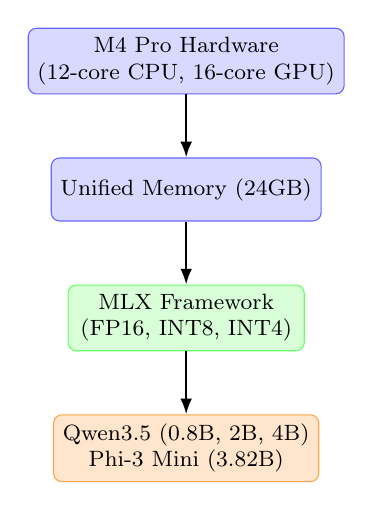
\begin{tikzpicture}[
    node distance=0.8cm,
    box/.style={
        rectangle,
        rounded corners=3pt,
        draw,
        minimum width=3cm,
        minimum height=0.8cm,
        align=center,
        font=\footnotesize
    },
    arrow/.style={
        -{Latex[length=2mm, width=1.5mm]},
        thick
    }
]
% === Hardware Layer ===
\node[box, fill=blue!15, draw=blue!60] (hardware) {M4 Pro Hardware\\(12-core CPU, 16-core GPU)};
\node[box, fill=blue!15, draw=blue!60, below=of hardware] (memory) {Unified Memory (24GB)};

% === Framework Layer ===
\node[box, fill=green!15, draw=green!60, below=0.8cm of memory] (mlx) {MLX Framework\\(FP16, INT8, INT4)};

% === Model Layer ===
\node[box, fill=orange!20, draw=orange!70, below=0.8cm of mlx] (models) {Qwen3.5 (0.8B, 2B, 4B)\\Phi-3 Mini (3.82B)};

% === Arrows ===
\draw[arrow] (hardware) -- (memory);
\draw[arrow] (memory) -- (mlx);
\draw[arrow] (mlx) -- (models);
\end{tikzpicture}
\caption{System architecture for PTQ evaluation on Apple Silicon using MLX.}
\label{fig:system_architecture}
\end{figure}

\begin{figure*}[htbp]
\centering
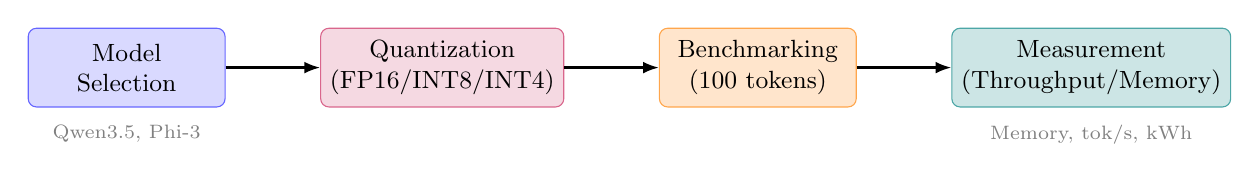
\begin{tikzpicture}[
    node distance=1.2cm,
    box/.style={
        rectangle,
        rounded corners=3pt,
        draw,
        minimum width=2.5cm,
        minimum height=1cm,
        align=center,
        font=\small
    },
    arrow/.style={
        -{Latex[length=2mm, width=1.5mm]},
        thick
    }
]
% Nodes (horizontal layout)
\node[box, fill=blue!15, draw=blue!60] (select) {Model\\Selection};
\node[box, fill=purple!15, draw=purple!60, right=of select] (quant) {Quantization\\(FP16/INT8/INT4)};
\node[box, fill=orange!20, draw=orange!70, right=of quant] (bench) {Benchmarking\\(100 tokens)};
\node[box, fill=teal!20, draw=teal!70, right=of bench] (measure) {Measurement\\(Throughput/Memory)};

% Arrows
\draw[arrow] (select) -- (quant);
\draw[arrow] (quant) -- (bench);
\draw[arrow] (bench) -- (measure);

% Labels below
\node[below=0.1cm of select, font=\scriptsize, text=gray] {Qwen3.5, Phi-3};
\node[below=0.1cm of measure, font=\scriptsize, text=gray] {Memory, tok/s, kWh};
\end{tikzpicture}
\caption{Experimental workflow for generation benchmarking on Apple Silicon. Accuracy is measured separately with a full logit-based MMLU pass.}
\label{fig:experimental_workflow}
\end{figure*}

Figure~\ref{fig:experimental_workflow} lays out the throughput, memory, and energy pipeline: pick a model, quantize it, benchmark generation, and collect the system metrics. Accuracy is evaluated separately using the full MMLU sweep described below.

\subsection{Models}

We picked these models for three reasons. First, \textbf{size diversity}: the Qwen3.5 series goes from 873M to 4.66B parameters, so we can see how model scale affects quantization trade-offs. Second, \textbf{they are genuinely good}: both families post strong benchmark numbers while staying small enough for edge hardware. Third, \textbf{architectural diversity}: Qwen3.5 uses GQA attention with RoPE embeddings, while Phi-3 is a straightforward dense transformer.

\subsubsection{Qwen3.5 Series}

The Qwen3.5 series \cite{qwen2025technical} from Alibaba are efficient language models with hybrid reasoning capabilities:

\begin{itemize}[leftmargin=*,nosep]
    \item \textbf{Qwen3.5-0.8B}: 873M parameters, optimized for extreme efficiency
    \item \textbf{Qwen3.5-2B}: 2.27B parameters, balanced size--performance trade-off
    \item \textbf{Qwen3.5-4B}: 4.66B parameters, higher accuracy with greater resource requirements
\end{itemize}

Key features include GQA attention, RoPE embeddings, SwiGLU activation, and dual-mode reasoning (thinking/non-thinking). All Qwen3.5 experiments were conducted using MLX.

\subsubsection{Phi-3 Mini}

Phi-3 Mini \cite{abdin2024phi3} is a 3.82-billion-parameter dense transformer from Microsoft: 3072 hidden dimensions, 32 attention heads, 32 layers, 128K context length. Experiments were conducted using MLX.

\subsection{Hardware Platform}

Everything runs on Apple Silicon. The M4 Pro's key feature for LLM inference is its unified memory, where CPU and GPU share the same physical RAM, eliminating data transfer bottlenecks. For models that are heavily memory-bandwidth-bound (which LLMs almost always are during generation), this makes a real difference. Full hardware specifications are in Section~\ref{sec:hw-setup}.

\subsection{Evaluation Metrics}

We measure four things for each model--quantization pair. Throughput and energy numbers are the mean of 10 runs after one warmup run. Accuracy is computed deterministically from a single full-MMLU sweep over the same 14,042 questions for every configuration. Standard deviations stayed below 3\% for throughput across all configurations. We omit error bars for readability but note this variability bound.

\subsubsection{Throughput}

We measure inference throughput during generation of 100 tokens with a 256-token input context:

\begin{equation}
\text{Throughput} = \frac{\text{Number of Tokens Generated}}{\text{Total Generation Time}}
\end{equation}

\subsubsection{Memory Footprint}

We measure peak memory consumption during inference, which includes model weights (quantized or full-precision), KV cache, activation buffers, and runtime overhead.

\subsubsection{Task Accuracy}

For accuracy, we use the full MMLU test split \cite{hendrycks2021mmlu}: all 57 subjects and 14,042 questions, grouped into STEM, Humanities, Social Sciences, and Other. We use \textbf{logit-based scoring}: for each multiple-choice question, we look at the model's next-token log-probabilities for A, B, C, and D, and pick the highest. It is deterministic, produces no unparseable responses, and matches the evaluation style used in lm-evaluation-harness \cite{eval-harness}.

At this sample size, the binomial 95\% confidence interval around overall accuracy is roughly $\pm 0.8$\,pp, tight enough to distinguish the multi-point INT4 drops we observe from ordinary sampling noise.

\subsubsection{Energy Estimation}
\label{sec:energy_method}

We estimate energy consumption using CodeCarbon \cite{codecarbon2023}:

\begin{equation}
E_{\text{inference}} = \int_{t_0}^{t_1} P(t) \, dt
\end{equation}

where $P(t)$ is instantaneous power consumption.

\textbf{Limitation}: CodeCarbon on Apple Silicon cannot read actual hardware power sensors (RAPL is Intel-only). It falls back to a TDP-based model that assumes roughly constant power draw (about 42.5\,W for the CPU and 6\,W for RAM). Because the estimated power is essentially a constant, \textbf{the energy numbers end up being roughly proportional to wall-clock time}. We include these numbers because they are still useful for rough comparisons, but they should not be taken as precise energy measurements. Real power data on Apple Silicon would require an external power meter or Apple's \texttt{powermetrics} with root access.

\subsection{Experimental Setup}

\subsubsection{Hardware}
\label{sec:hw-setup}

All experiments were conducted on:
\begin{itemize}[leftmargin=*,nosep]
    \item \textbf{Platform}: Apple MacBook Pro (M4 Pro)
    \item \textbf{Processor}: Apple M4 Pro (12-core CPU, 16-core GPU)
    \item \textbf{Memory}: 24\,GB unified memory (LPDDR5X)
    \item \textbf{Storage}: 512\,GB SSD
    \item \textbf{OS}: macOS Sequoia 15.3
\end{itemize}

\subsubsection{Software}

\begin{itemize}[leftmargin=*,nosep]
    \item \textbf{Framework}: MLX 0.31.0 (Apple-native)
    \item \textbf{Quantization}: MLX built-in quantization (FP16, INT8, INT4)
    \item \textbf{Energy estimation}: CodeCarbon 3.2.3
    \item \textbf{Accuracy evaluation}: Custom logit-based MMLU scorer using Hugging Face Transformers
\end{itemize}

\subsubsection{Benchmarking Protocol}

\begin{itemize}[leftmargin=*,nosep]
    \item Generation length: 100 tokens
    \item Input context: 256 tokens
    \item Temperature: 0.0 (greedy decoding)
    \item Warmup: 1 run (discarded) before 10 measured runs
    \item Accuracy benchmark: full MMLU test split (57 subjects, 14,042 questions) scored by next-token logits over A/B/C/D
    \item Random seed: 42 for reproducibility
    \item Thinking mode: disabled for Qwen3.5 models during generation and MMLU scoring
\end{itemize}

% =============================================================================
% 5. EXPERIMENTS AND RESULTS
% =============================================================================
\section{Experiments and Results}

Here are the results from running all four models through MLX at three precision levels (FP16, INT8, INT4) on our M4 Pro. Throughput and energy numbers are averages of 10 runs after a warmup pass; accuracy numbers come from a single deterministic sweep over the full 14,042-question MMLU test set.

\subsection{Memory Footprint}

Table~\ref{tab:memory} shows memory requirements across all configurations.

\begin{table}[htbp]
\centering
\caption{Memory footprint (GB) across MLX quantization levels.}
\label{tab:memory}
\begin{tabular}{l|ccc}
\toprule
\textbf{Model} & \textbf{FP16} & \textbf{INT8} & \textbf{INT4} \\
\midrule
Qwen3.5-0.8B & 1.40 & 0.74 & 0.39 \\
Qwen3.5-2B & 3.51 & 1.86 & 0.99 \\
Qwen3.5-4B & 7.83 & 4.16 & 2.20 \\
Phi-3 Mini & 7.12 & 3.78 & 2.00 \\
\bottomrule
\end{tabular}
\end{table}

INT4 delivers $3.5\times$--$3.6\times$ memory reduction over FP16 across the board. Every model fits within 2.5\,GB at INT4, making edge deployment feasible even on devices with only 8\,GB of RAM.

\subsection{Quantization Method Comparison}

Table~\ref{tab:quant_comparison} compares quantization configurations for Qwen3.5-0.8B.

\begin{table}[htbp]
\centering
\caption{Quantization comparison for Qwen3.5-0.8B on M4 Pro (100 tokens generated).}
\label{tab:quant_comparison}
\begin{tabular}{l|cccc}
\toprule
\textbf{Method} & \textbf{Size (GB)} & \textbf{tok/s} & \textbf{ms/tok} & \textbf{Speedup} \\
\midrule
FP16 & 1.40 & 104.69 & 9.55 & 1.0$\times$ \\
INT8 & 0.74 & 166.08 & 6.02 & 1.6$\times$ \\
INT4 & 0.39 & 213.11 & 4.69 & 2.0$\times$ \\
\bottomrule
\end{tabular}
\end{table}

The pattern is clean: lower bit-width means higher throughput. INT4 runs $2.0\times$ faster than FP16 for this model, with INT8 sitting in between at $1.6\times$. Each step down in precision roughly halves memory while boosting throughput.

\subsection{Throughput Analysis}

Table~\ref{tab:latency} presents throughput and memory across all MLX configurations.

\begin{table*}[htbp]
\centering
\caption{MLX throughput and memory across quantization levels (100 tokens generated).}
\label{tab:latency}
\resizebox{\textwidth}{!}{%
\begin{tabular}{l|ccccccc}
\toprule
\textbf{Model} & \multicolumn{2}{c}{\textbf{FP16}} & \multicolumn{2}{c}{\textbf{INT8}} & \multicolumn{2}{c}{\textbf{INT4}} & \textbf{Speedup} \\
\cmidrule(lr){2-3} \cmidrule(lr){4-5} \cmidrule(lr){6-7}
& tok/s & GB & tok/s & GB & tok/s & GB & (INT4/FP16) \\
\midrule
Qwen3.5-0.8B & 104.69 & 1.40 & 166.08 & 0.74 & 213.11 & 0.39 & 2.0$\times$ \\
Qwen3.5-2B & 52.08 & 3.51 & 87.42 & 1.86 & 131.86 & 0.99 & 2.5$\times$ \\
Qwen3.5-4B & 24.15 & 7.83 & 42.49 & 4.16 & 71.21 & 2.20 & 2.9$\times$ \\
Phi-3 Mini & 23.23 & 7.12 & 45.64 & 3.78 & 88.40 & 2.00 & 3.8$\times$ \\
\bottomrule
\end{tabular}%
}
\end{table*}

\begin{figure}[htbp]
\centering
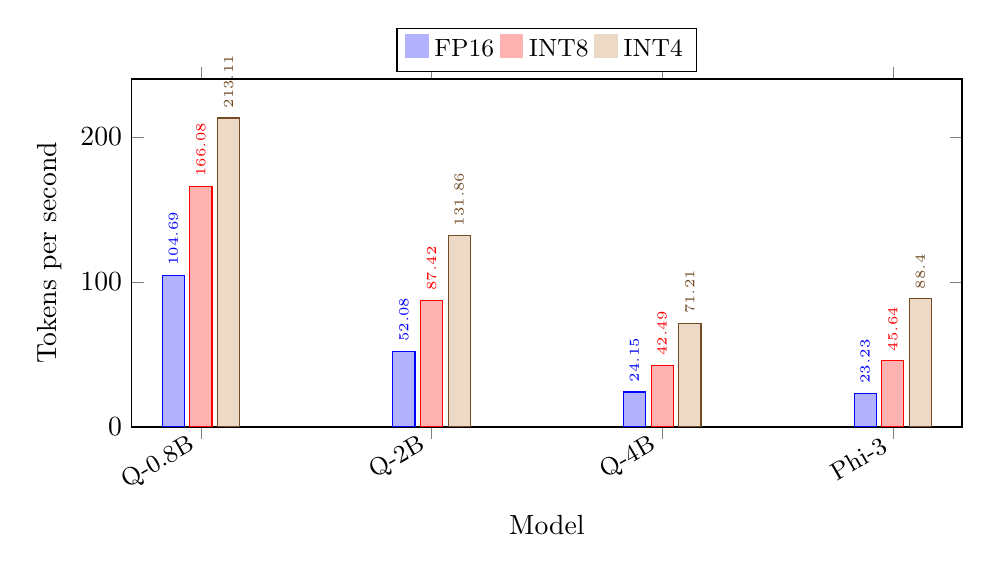
\begin{tikzpicture}
\begin{axis}[
    ybar,
    bar width=8pt,
    width=\columnwidth,
    height=6cm,
    ylabel={Tokens per second},
    xlabel={Model},
    symbolic x coords={Q-0.8B, Q-2B, Q-4B, Phi-3},
    xtick=data,
    x tick label style={rotate=30, anchor=east, font=\small},
    ymin=0,
    ymax=240,
    legend style={at={(0.5,1.02)}, anchor=south, legend columns=3, font=\small},
    legend image code/.code={\draw[fill,draw=none,#1] (0cm,-0.1cm) rectangle (0.3cm,0.2cm);},
    nodes near coords,
    nodes near coords style={font=\tiny},
    every node near coord/.append style={rotate=90, anchor=west}
]
\addplot coordinates {(Q-0.8B,104.69) (Q-2B,52.08) (Q-4B,24.15) (Phi-3,23.23)};
\addplot coordinates {(Q-0.8B,166.08) (Q-2B,87.42) (Q-4B,42.49) (Phi-3,45.64)};
\addplot coordinates {(Q-0.8B,213.11) (Q-2B,131.86) (Q-4B,71.21) (Phi-3,88.40)};
\legend{FP16, INT8, INT4}
\end{axis}
\end{tikzpicture}
\caption{MLX throughput across quantization levels. Larger models exhibit greater relative speedup from INT4 quantization, likely because they are more memory-bandwidth-bound at FP16.}
\label{fig:tokens_per_sec}
\end{figure}

Two things jump out from Table~\ref{tab:latency} and Figure~\ref{fig:tokens_per_sec}. First, the bigger the model, the more you gain from INT4: the speedup goes from $2.0\times$ for the 0.8B model up to $3.8\times$ for Phi-3 Mini. This makes sense because larger models are more memory-bandwidth-bound at FP16, so cutting bandwidth by $4\times$ helps them more. Second, Phi-3 Mini (3.82B) actually runs faster at INT4 (88.40\,tok/s) than the larger Qwen3.5-4B (71.21\,tok/s, 4.66B), likely because Phi-3's simpler dense architecture is more compute-efficient per parameter.

\subsection{Energy Estimation}

We reiterate the caveat from Section~\ref{sec:energy_method}: on Apple Silicon, CodeCarbon's energy numbers are derived from TDP-based power models and track inference time more than actual power draw. Table~\ref{tab:mlx_energy} shows the estimated energy across MLX quantization levels.

\begin{table*}[htbp]
\centering
\caption{MLX estimated energy across quantization levels (100 tokens). Energy values are CodeCarbon estimates based on TDP models, not direct measurements.}
\label{tab:mlx_energy}
\resizebox{\textwidth}{!}{%
\begin{tabular}{l|ccccccc}
\toprule
\textbf{Model} & \multicolumn{2}{c}{\textbf{FP16}} & \multicolumn{2}{c}{\textbf{INT8}} & \multicolumn{2}{c}{\textbf{INT4}} & \textbf{Est.\ Energy} \\
\cmidrule(lr){2-3} \cmidrule(lr){4-5} \cmidrule(lr){6-7}
& tok/s & kWh & tok/s & kWh & tok/s & kWh & Ratio \\
\midrule
Qwen3.5-0.8B & 104.69 & 0.000013 & 166.08 & 0.000008 & 213.11 & 0.000006 & 2.2$\times$ \\
Qwen3.5-2B & 52.08 & 0.000026 & 87.42 & 0.000015 & 131.86 & 0.000010 & 2.6$\times$ \\
Qwen3.5-4B & 24.15 & 0.000056 & 42.49 & 0.000032 & 71.21 & 0.000019 & 2.9$\times$ \\
Phi-3 Mini & 23.23 & 0.000058 & 45.64 & 0.000030 & 88.40 & 0.000015 & 3.9$\times$ \\
\bottomrule
\end{tabular}%
}
\end{table*}

\begin{figure}[htbp]
\centering
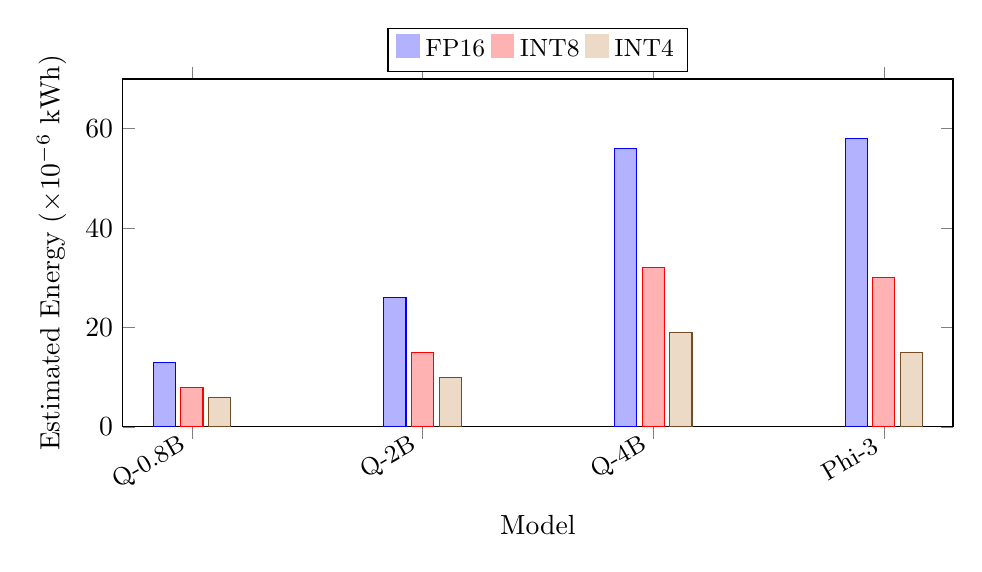
\begin{tikzpicture}
\begin{axis}[
    ybar,
    bar width=8pt,
    width=\columnwidth,
    height=6cm,
    ylabel={Estimated Energy ($\times 10^{-6}$ kWh)},
    xlabel={Model},
    symbolic x coords={Q-0.8B, Q-2B, Q-4B, Phi-3},
    xtick=data,
    x tick label style={rotate=30, anchor=east, font=\small},
    ymin=0,
    ymax=70,
    legend style={at={(0.5,1.02)}, anchor=south, legend columns=3, font=\small},
    legend image code/.code={\draw[fill,draw=none,#1] (0cm,-0.1cm) rectangle (0.3cm,0.2cm);}
]
\addplot coordinates {(Q-0.8B,13) (Q-2B,26) (Q-4B,56) (Phi-3,58)};
\addplot coordinates {(Q-0.8B,8) (Q-2B,15) (Q-4B,32) (Phi-3,30)};
\addplot coordinates {(Q-0.8B,6) (Q-2B,10) (Q-4B,19) (Phi-3,15)};
\legend{FP16, INT8, INT4}
\end{axis}
\end{tikzpicture}
\caption{Estimated energy consumption across MLX quantization levels. Because CodeCarbon uses constant TDP-based power estimates on Apple Silicon, these values are approximately proportional to inference time (see Section~\ref{sec:energy_method}).}
\label{fig:energy_quantization}
\end{figure}

\subsection{Accuracy Retention Under Quantization}
\label{sec:accuracy}

Table~\ref{tab:mmlu_accuracy} presents full MMLU accuracy across all models and quantization levels, measured using logit-based scoring on all 57 subjects (14,042 questions).

\begin{table*}[htbp]
\centering
\caption{Full MMLU accuracy (\%) across quantization levels (logit-based scoring, all 57 subjects, $n=14{,}042$). Binomial 95\% confidence intervals around overall accuracy are approximately $\pm 0.8$\,pp.}
\label{tab:mmlu_accuracy}
\resizebox{\textwidth}{!}{%
\begin{tabular}{l l c c c c c}
\toprule
\textbf{Model} & \textbf{Quant} & \textbf{Overall} & \textbf{STEM} & \textbf{Human.} & \textbf{Social} & \textbf{Other} \\
\midrule
Qwen3.5-0.8B & FP16 & 46.31 & 44.50 & 39.06 & 52.63 & 52.88 \\
Qwen3.5-0.8B & INT8 & 45.27 & 42.63 & 38.66 & 51.12 & 52.21 \\
Qwen3.5-0.8B & INT4 & 43.73 & 40.50 & 38.13 & 50.02 & 49.22 \\
Qwen3.5-2B & FP16 & 56.59 & 53.95 & 49.39 & 64.40 & 62.35 \\
Qwen3.5-2B & INT8 & 56.54 & 53.92 & 49.03 & 64.34 & 62.82 \\
Qwen3.5-2B & INT4 & 48.68 & 45.67 & 42.44 & 54.99 & 54.94 \\
Qwen3.5-4B & FP16 & 73.11 & 70.38 & 66.16 & 81.11 & 78.38 \\
Qwen3.5-4B & INT8 & 73.07 & 70.31 & 66.18 & 80.96 & 78.42 \\
Qwen3.5-4B & INT4 & 69.82 & 66.48 & 61.64 & 79.10 & 76.32 \\
Phi-3 Mini & FP16 & 69.36 & 61.72 & 64.00 & 79.07 & 75.52 \\
Phi-3 Mini & INT8 & 69.29 & 61.91 & 63.93 & 78.88 & 75.29 \\
Phi-3 Mini & INT4 & 66.97 & 59.44 & 62.02 & 76.49 & 72.56 \\
\bottomrule
\end{tabular}%
}
\end{table*}

\begin{figure}[htbp]
\centering
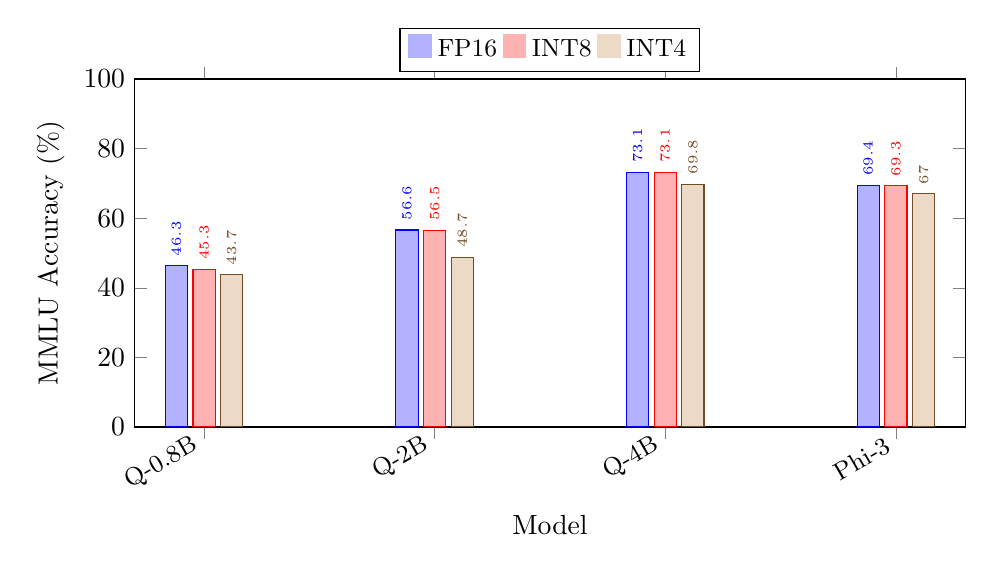
\begin{tikzpicture}
\begin{axis}[
    ybar,
    bar width=8pt,
    width=\columnwidth,
    height=6cm,
    ylabel={MMLU Accuracy (\%)},
    xlabel={Model},
    symbolic x coords={Q-0.8B, Q-2B, Q-4B, Phi-3},
    xtick=data,
    x tick label style={rotate=30, anchor=east, font=\small},
    ymin=0,
    ymax=100,
    legend style={at={(0.5,1.02)}, anchor=south, legend columns=3, font=\small},
    legend image code/.code={\draw[fill,draw=none,#1] (0cm,-0.1cm) rectangle (0.3cm,0.2cm);},
    nodes near coords,
    nodes near coords style={font=\tiny},
    every node near coord/.append style={rotate=90, anchor=west}
]
\addplot coordinates {(Q-0.8B,46.3) (Q-2B,56.6) (Q-4B,73.1) (Phi-3,69.4)};
\addplot coordinates {(Q-0.8B,45.3) (Q-2B,56.5) (Q-4B,73.1) (Phi-3,69.3)};
\addplot coordinates {(Q-0.8B,43.7) (Q-2B,48.7) (Q-4B,69.8) (Phi-3,67.0)};
\legend{FP16, INT8, INT4}
\end{axis}
\end{tikzpicture}
\caption{MMLU accuracy across quantization levels on the full 57-subject test set ($n=14{,}042$). The larger sample makes the INT4 degradation clear, while INT8 remains nearly lossless for the 2B and larger models.}
\label{fig:mmlu_accuracy}
\end{figure}

With $n=14{,}042$, overall accuracy has a 95\% confidence interval of roughly $\pm 0.8$\,pp, so the INT4 drops are no longer explainable as small-sample noise. The data shows:

\begin{enumerate}[leftmargin=*,nosep]
    \item \textbf{INT8 is essentially lossless for the 2B and larger models}: relative to FP16, the drop is just 0.04\,pp for Qwen3.5-2B, 0.04\,pp for Qwen3.5-4B, and 0.07\,pp for Phi-3 Mini. Qwen3.5-0.8B is the only model with a clearly visible INT8 shift (1.04\,pp).

    \item \textbf{INT4 introduces real but model-dependent degradation}: the full-MMLU drop is 2.59\,pp for Qwen3.5-0.8B, 7.90\,pp for Qwen3.5-2B, 3.29\,pp for Qwen3.5-4B, and 2.39\,pp for Phi-3 Mini.

    \item \textbf{Category structure is stable under quantization}: Social Sciences is the strongest category for every configuration. The largest INT4 degradation appears in Qwen3.5-2B, where all category drops fall between 6.95 and 9.41\,pp.

    \item \textbf{Accuracy still scales with model quality}: within the Qwen3.5 family, FP16 accuracy rises from 46.31\% to 56.59\% to 73.11\%. INT4 follows the same pattern, rising from 43.73\% to 48.68\% to 69.82\%.
\end{enumerate}

\subsection{Energy--Accuracy Trade-off}

We define \textit{accuracy depreciation} as the full-MMLU drop relative to the FP16 baseline and \textit{estimated energy reduction} as $100 \times (1 - E_q/E_{\text{FP16}})$. Figure~\ref{fig:energy_accuracy_tradeoff} plots these two deltas together.

\begin{figure}[htbp]
\centering
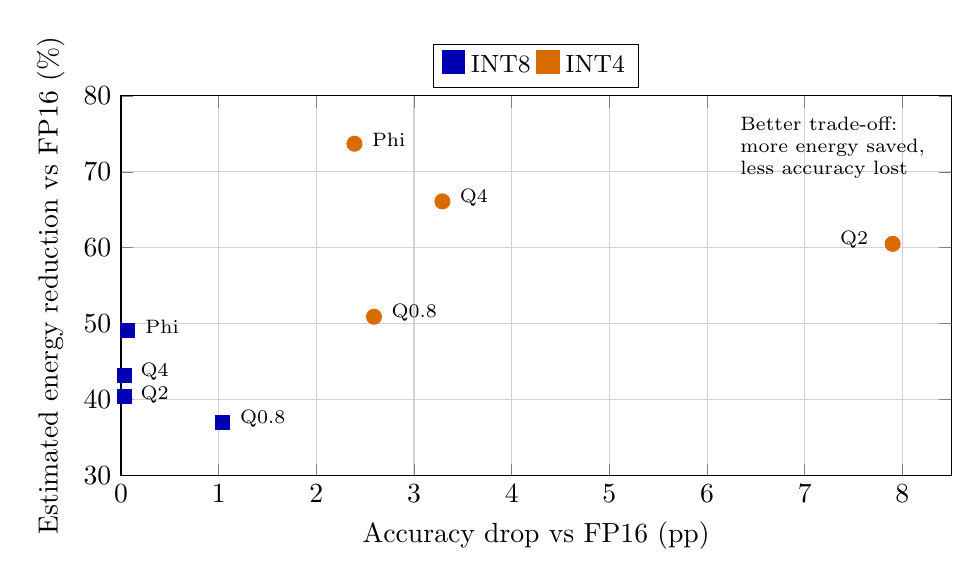
\begin{tikzpicture}
\begin{axis}[
    width=\columnwidth,
    height=6.4cm,
    xlabel={Accuracy drop vs FP16 (pp)},
    ylabel={Estimated energy reduction vs FP16 (\%)},
    xmin=0,
    xmax=8.5,
    ymin=30,
    ymax=80,
    xtick={0,1,2,3,4,5,6,7,8},
    ytick={30,40,50,60,70,80},
    grid=both,
    grid style={gray!20},
    major grid style={gray!35},
    legend style={at={(0.5,1.02)}, anchor=south, legend columns=2, font=\small},
    legend image code/.code={\draw[fill,draw=none,#1] (0cm,-0.1cm) rectangle (0.3cm,0.2cm);}
]
\addplot[only marks, mark=square*, mark size=2.5pt, blue!70!black] coordinates {
    (1.04,36.9)
    (0.04,40.4)
    (0.04,43.2)
    (0.07,49.1)
};
\addplot[only marks, mark=*, mark size=2.7pt, orange!85!black] coordinates {
    (2.59,50.9)
    (7.90,60.5)
    (3.29,66.1)
    (2.39,73.7)
};
\legend{INT8, INT4}

\node[font=\scriptsize, anchor=west] at (axis cs:0.10,40.6) {Q2};
\node[font=\scriptsize, anchor=west] at (axis cs:0.10,43.7) {Q4};
\node[font=\scriptsize, anchor=west] at (axis cs:0.15,49.6) {Phi};
\node[font=\scriptsize, anchor=west] at (axis cs:1.12,37.4) {Q0.8};

\node[font=\scriptsize, anchor=west] at (axis cs:2.47,74.2) {Phi};
\node[font=\scriptsize, anchor=west] at (axis cs:2.67,51.4) {Q0.8};
\node[font=\scriptsize, anchor=west] at (axis cs:3.37,66.6) {Q4};
\node[font=\scriptsize, anchor=east] at (axis cs:7.75,61.0) {Q2};

\node[font=\scriptsize, align=left, anchor=north east] at (rel axis cs:0.98,0.97) {Better trade-off:\\more energy saved,\\less accuracy lost};
\end{axis}
\end{tikzpicture}
\caption{Energy--accuracy trade-off relative to each model's FP16 baseline. Upper-left points are preferable: less full-MMLU accuracy loss for more estimated energy reduction. INT8 occupies the low-loss region; Phi-3 Mini INT4 and Qwen3.5-4B INT4 offer the strongest aggressive-quantization trade-offs.}
\label{fig:energy_accuracy_tradeoff}
\end{figure}

INT8 for Qwen3.5-2B, Qwen3.5-4B, and Phi-3 Mini sits in the low-loss, high-gain corner, cutting estimated energy by 40.4--49.1\% while losing at most 0.07\,pp on full MMLU. Among INT4 configurations, Phi-3 Mini gives the strongest result: 73.7\% lower estimated energy for a 2.39\,pp accuracy drop. The clear outlier is Qwen3.5-2B INT4, which saves 60.5\% energy but pays with the largest accuracy depreciation in the study (7.90\,pp).

\subsection{Experimental Limitations}

\begin{enumerate}[leftmargin=*,nosep]
    \item \textbf{Energy estimation}: CodeCarbon on Apple Silicon uses TDP-based power models. Energy values correlate strongly with inference time rather than direct power measurements.

    \item \textbf{Benchmark coverage}: Full MMLU does not measure open-ended generation quality, coding, tool use, safety, or long-context reasoning.

    \item \textbf{Single device}: All results are from a single M4 Pro unit; chip-to-chip variation and thermal throttling under sustained load are not characterized.

    \item \textbf{Short generation length}: Benchmarks use 100-token generation; throughput and energy characteristics may differ for longer sequences or batched inference.
\end{enumerate}

\subsection{Recommendations for Practitioners}

\begin{enumerate}[leftmargin=*,nosep]
    \item \textbf{Quantization level}: INT4 provides the best throughput--memory trade-off for 4B-class models when a 2--3\,pp MMLU drop is acceptable (Figure~\ref{fig:energy_accuracy_tradeoff}). For smaller models or accuracy-sensitive deployments, INT8 is the safer default.

    \item \textbf{Model selection}: Qwen3.5-4B offers the best absolute accuracy at every precision, while Phi-3 Mini INT4 delivers the strongest aggressive energy--accuracy trade-off: 73.7\% estimated energy reduction for only a 2.39\,pp MMLU drop.
\end{enumerate}

% =============================================================================
% 6. DISCUSSION
% =============================================================================
\section{Discussion}

\subsection{Why Unified Memory Matters}

Apple Silicon's unified memory architecture is not just a marketing feature. When CPU and GPU share the same memory pool, reducing weight precision translates directly into less memory bandwidth consumed. Since memory bandwidth is the bottleneck for autoregressive generation, this matters greatly. This is why the INT4 speedup ratio increases with model size (Table~\ref{tab:latency}): bigger models are more bandwidth-starved at FP16, so they benefit more from the $4\times$ bandwidth reduction INT4 provides. Benazir and Lin \cite{benazir2025profiling} found independently that Apple Silicon amplifies quantization benefits compared to discrete-GPU systems.

\subsection{The Accuracy Question}

Our full MMLU results sharpen the answer. INT8 is essentially free for the 2B and larger models: the change from FP16 is only 0.04\,pp for Qwen3.5-2B and Qwen3.5-4B, and 0.07\,pp for Phi-3 Mini. INT4 is a different story. The accuracy loss is real for every model, but its magnitude depends strongly on the model: 2.59\,pp for Qwen3.5-0.8B, 7.90\,pp for Qwen3.5-2B, 3.29\,pp for Qwen3.5-4B, and 2.39\,pp for Phi-3 Mini.

This result is important because it means there is no magic parameter threshold where INT4 suddenly becomes free. Scale helps, but architecture and training recipe matter too. This broadly aligns with what Kurtic et al.\ \cite{kurtic2024give} and Jin et al.\ \cite{jin2024comprehensive} reported: quantization sensitivity is model-dependent rather than determined by bit-width alone.

\subsection{The Energy Measurement Problem}

CodeCarbon's TDP model assumes roughly constant power draw, which is an approximation. During steady-state token generation, the M4 Pro is probably pulling a fairly consistent amount of power regardless of weight precision, since the chip still saturates its memory bus either way. If that assumption holds, faster inference really does mean less energy per token, and our estimates are directionally correct even if the exact numbers are off.

The interesting open question is whether INT4 workloads actually use \textit{less} power than FP16 at the hardware level. INT4 needs fewer compute operations but similar memory bandwidth. We flag this as one of the most valuable directions for future work.

\subsection{Limitations}

\subsubsection{Hardware Specificity}

Everything we measured is specific to one chip, the M4 Pro. NVIDIA GPUs with separate VRAM may show different trade-offs due to PCIe bottlenecks; mobile SoCs have less memory and different thermal profiles; results may not generalize to other Apple Silicon variants.

\subsubsection{Model Coverage}

We only tested four models from two families. Qwen3.5 thinking mode was disabled; enabling it may affect quantization sensitivity. Mixture-of-Expert architectures and models larger than 5B parameters were not evaluated.

\subsection{Future Work}

\begin{enumerate}[leftmargin=*,nosep]
    \item \textbf{Hardware power measurement}: Using external power meters or Apple's \texttt{powermetrics} to obtain ground-truth energy data on Apple Silicon.

    \item \textbf{Broader benchmark coverage}: Extending evaluation beyond MMLU to reasoning, coding, long-context, and open-ended generation benchmarks.

    \item \textbf{Cross-architecture evaluation}: Extending experiments to NVIDIA GPUs, mobile NPUs, and embedded processors.

    \item \textbf{Dynamic quantization}: Exploring per-layer or per-block adaptive bit-width selection based on sensitivity analysis.

    \item \textbf{Combined techniques}: Evaluating quantization combined with structured pruning or knowledge distillation for further compression.
\end{enumerate}

% =============================================================================
% 7. CONCLUSION
% =============================================================================
\section{Conclusion}

We evaluated post-training quantization for deploying small language models on Apple Silicon. We ran the Qwen3.5 series (0.8B, 2B, 4B) and Phi-3 Mini through MLX at three precision levels (FP16, INT8, INT4) on an M4 Pro with 24\,GB of unified memory.

\begin{enumerate}[leftmargin=*,nosep]
    \item \textbf{Throughput}: INT4 provides $2.0\times$--$3.8\times$ throughput improvement over FP16, with speedup increasing with model size.

    \item \textbf{Memory efficiency}: INT4 delivers $3.5\times$--$3.6\times$ memory reduction, with all models fitting within 2.5\,GB, enabling deployment on devices with 8\,GB RAM.

    \item \textbf{Full-MMLU accuracy}: On all 57 subjects (14,042 questions), INT8 is effectively lossless for the 2B and larger models, while INT4 causes measurable drops of 2.39--7.90\,pp depending on the model. The 4B-class models absorb INT4 best, losing 2.39--3.29\,pp overall.
\end{enumerate}

On Apple Silicon, INT4 quantization via MLX is the best speed--memory option when a modest accuracy trade-off is acceptable, especially for 4B-class models. When accuracy is the primary constraint, INT8 is the safer near-lossless default. The broader lesson is that aggressive quantization should be chosen per model, not per bit-width alone.

\begin{sloppypar}
\noindent\textbf{Code and Data:} Available at \url{https://github.com/harshpreet931/researchPaper-quantization}
\end{sloppypar}

% =============================================================================
% DECLARATION ON GENERATIVE AI
% =============================================================================
\section*{Declaration on Generative AI}

The authors used large language model (LLM) assistance for grammar checking and language refinement during the preparation of this manuscript. The development of scientific ideas, experimental design, data collection, analysis, results, and conclusions was carried out exclusively by the human authors. All AI-assisted text was critically reviewed and edited by the authors, who take full responsibility for the accuracy, originality, and integrity of this work. No generative AI tool is listed as an author.

% =============================================================================
% ACKNOWLEDGMENTS
% =============================================================================
\section*{Acknowledgments}

The authors acknowledge the developers of Hugging Face Transformers, CodeCarbon, and the Apple MLX team for making their tools openly available.

% =============================================================================
% REFERENCES
% =============================================================================
\bibliography{references}

\end{document}
